\documentclass{scrartcl}
\usepackage[utf8]{inputenc}
\usepackage{pgf-pie}
\usepackage{subfigure}
\usepackage{hyperref}
\usepackage{cite}
\usepackage{amsmath}
\usepackage{amssymb}
\usepackage{graphicx}
%\documentclass{book}
\renewcommand\thesubsection{\Alph{subsection}}


%opening
\title{Assignment 2}
\author{Daan Spijkers, s1011382\\ Tomás Catalán López, s1081589\\ Willem Lambooy, s1009584}

\begin{document}
\maketitle

\textbf{Note: you can find the GitHub repository at}
\url{github.com/dspkio/nacu}.

\section{Exercise 1}
\subsection{}
The code for this is in the notebook Assignment2\_1. After running it we get that the fitness of particles $x_1$, $x_2$ and $x_3$ is 730.35, 807.91 and 829.01

\subsection{}
In figure \ref{fig:1l} we can see how much each point has moved. For more detail, look into the notebook.

\begin{figure}[h!]
    \centering
    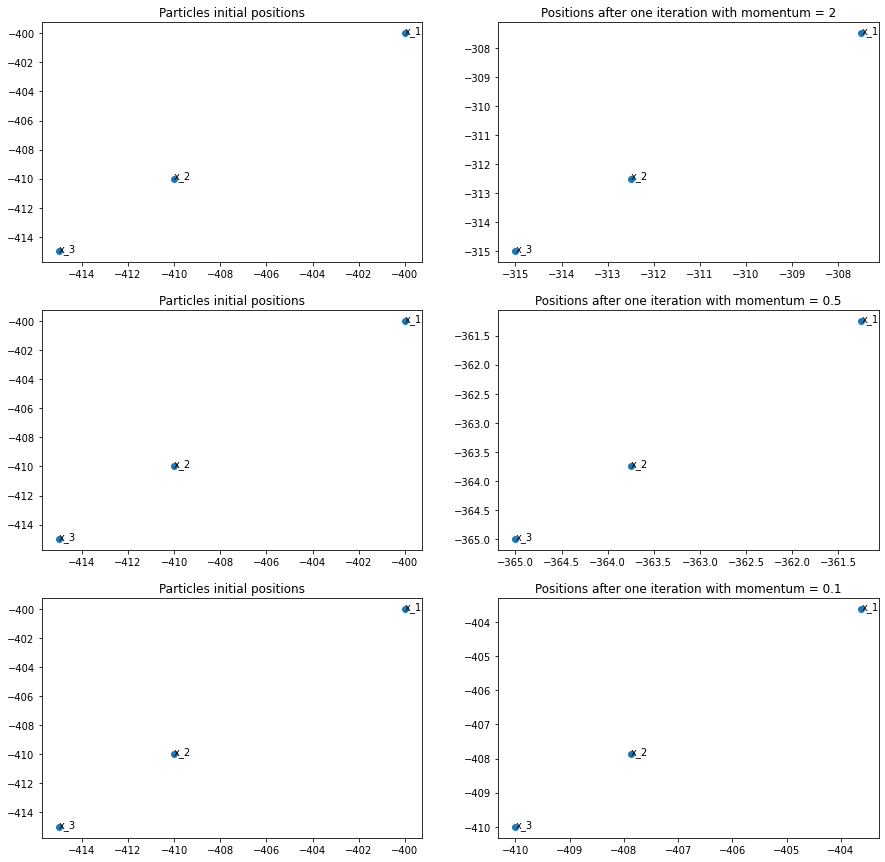
\includegraphics[width=0.65\textwidth]{images/1.png}
    \caption{Scatterplot of $x_1$, $x_2$ and $x_3$ after 1 iteration}
    \label{fig:1l}
\end{figure}

\subsection{}
The momentum has the function to "tune" the position of the particles. If it's $<1$, the best particle will be decreasing its velocity while it's approaxing a better position. If it's $>1$, the particle will be accelerating constantly.

\subsection{}
If we have a higher w, the particles will be moving faster, so it'd be easier to find the optimum if it's far away from the initial position, but it'll be hard to adjust it perfectly in a few iterations, so the computation will take longer.
On the other hand if we have a low momentum the particles would be able to adjust well to the optimum, but they may stop before reaching it (We can see this in Exercise 2.c).

\section{Exercise 2}
\subsection*{A. \& B.}
For the code, see the notebook \emph{assignment2\_1}.
See figure \ref{fig:2_1} for (a) and (b). With the first configuration,
the particle converges to the position $x = 15.0$, and for the second
configuration, the particle converges to the position $x = -100.34$.

\begin{figure}
  \centering
  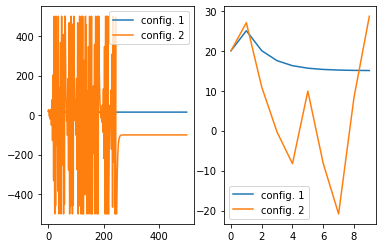
\includegraphics[width=0.65\textwidth]{images/2.png}
  \caption{2(a) and 2(b)}
  \label{fig:2_1}
\end{figure}

\subsection*{C.}
If we consider a single member swarm, the formula for calculating the
velocity of a particle i becomes like this:

It's only 1 particle so the personal best of the particle is also the
global best so:
\begin{align}
  & x_{i}^{*} = x^* \\
  & v_i = w*v_i + \alpha _1 r_1 (x^{*} - x_i) + \alpha _2 r_2 (x^{*} - x_i)
\end{align}

So if we have a w<1, that is always decreasing the velocity that the
particle has at any moment. We can see what would happen in the previous
plot in figure \ref{fig:2c}

\begin{figure}
  \centering
  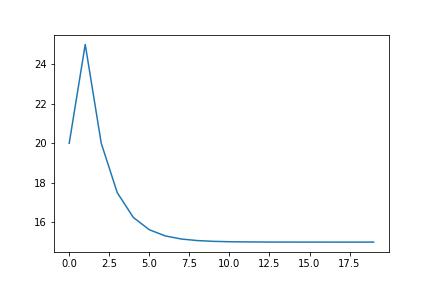
\includegraphics[width=0.65\textwidth]{images/2c.png}
  \caption{2(c)}
  \label{fig:2c}
\end{figure}

At first we can see a "bounce", because $\alpha _1 r_1 (x^{*} - x_i) + \alpha _2 r_2 (x^{*} - x_i)$ will be opossite to the velocity that it has at that moment, and afterwards the particle keeps moving to the optimum, so for each iteration we have:

$x^{*} = x_i \rightarrow v_i = w*v_i +0 +0 \rightarrow v_i = w*v_i$

The particle at that point is having its velocity decreased because of w, so it ends up stopping (In the former case before reaching the global optimum)

\section*{4.}

\begin{itemize}

  \item[(a)]
    No, it is not. Our space of valid solutions is $\{\{e_1, e_2\}, \{e_2,
    e_3\}, \{e_3, e_4\}\}$. We see that $e_1$ and $e_4$ occur only once,
    and $e_2$, $e_3$ occur twice.

  \item[(b)]
    Not always. Our goal is finding the optimal solution as efficiently as
    possible, if a bias is helpful for that then it is not harmful. If,
    for example, in the example given in (a) the weights for $e_2$ and
    $e_3$ were \emph{less} than the weights for $e_1$ and $e_4$, then this
    would be a positive thing.

\end{itemize}

\section*{5.}
The intuitive understanding is that ants going up will get a path straight
to the destination, while ants going down will get stuck, and have longer
paths. Even though the shortest path (length $5$) is down, it is possible
that the ants will converge on the upper path (length $8$).

If we calculate the expected length of the paths, then we can use that as
an indication for what the ant colony could converge on (the shorter the
expected length, the more pheromone). For the up path,
it is obvious that $E(up) = 9$.

For the down path, we can provide a lower bound by enumerating the
probabilities for all paths shorter than 9, and leaving all other paths
with length \emph{at least 10}.
\begin{equation}
  6  P(6) + 7  P(7) + 8  P(8) + 9  P(9) + 10(1 - P(\le9)) \le E(down)
\end{equation}

In the next section we assume that we initially go down. Describing the
enumeration is a bit cumbersome, but please bear with us. For the shortest
path of length 6 we need to choose the correct middle one at the 3rd
vertex (out of 3 choices), and then choose correctly again at the 4th and
5th vertex. This gives it $P(6) = \frac{1}{3} \times \frac{1}{2} \times
\frac{1}{2} = \frac{1}{12}$.

Length 7 is the exact same. For length 8 we can have a similar one of
probability $\frac{1}{12}$, but another way is to have the same initial
path of length 6, but then "miss" the 4th one, and then choose
correctly twice after that. This gives it $P(8) = \frac{1}{12} +
\frac{1}{48}$. Similarly, $P(9) = \frac{1}{48}$, as we can only get it by
"missing" once in the 7 length path. Now, $P(>9) = 1 - \frac{2}{12} -
\frac{2}{48} = \frac{19}{24}$, and the lower bound is:

\begin{equation}
  10 = \frac{6}{12} + \frac{7}{12} + 8(\frac{1}{12} + \frac{1}{48}) +
  \frac{9}{48} + 10 \times \frac{19}{24} \le E(down)
\end{equation}

So, the expected length for paths going down is at least $1$ higher
than the expected length for paths going up. This means it is quite
possible for things to converge on the up path. This is still random,
obviously, and so it will depend on the randomness and exact parameters of
the algorithm which path it will actually find.

\end{document}
